\documentclass[twocolumn, aps, floatfix]{revtex4-1}

\usepackage{graphicx}
\usepackage{fancyhdr}
\usepackage{amssymb}
\usepackage{amsmath}
\usepackage{caption}
\usepackage{enumerate}
\usepackage{subcaption}
\usepackage{textcomp}
\usepackage{placeins}
\usepackage{blindtext}

\begin{document}
\title{Lab 4. Balanced Mixers }
\author{Albert Wandui}
\affiliation{EE 152: High Frequency Systems Lab.}
\maketitle

\section*{Introduction}\label{sec:introduction}

The goal of this lab was to design, fabricate and characterize the performance of a balanced microwave mixer operating at 5.9 GHz. Mixer circuits are used to perform frequency translation, converting input at a given frequency and ideally producing an output at a single other frequency. The input is usually referred to as the RF (Radio Frequency) input and the output is the IF (Intermediate Frequency). In addition, a third signal, the local oscillator (LO) is used to perform the frequency translation. 

Mathematically, assuming that the RF input is at a single frequency, we can describe the input signal, $V_{in}(t)$ as $V_{in}(t) = V_{RF} \cos\left(\omega_{RF}\ t + \phi_{RF} \right)$. Similarly, the local oscillator can be written as $V_{LO}\cos \left(\omega_{LO} t \right)$. Here, I've set the phase of the LO to zero without loss of generality since we are only interested in the relative phase between RF and LO. For a multiplicative mixer, the output signal is proportional to the product of the RF and LO signals. Thus we can write,

\begin{align*}
    V_{out}(t) & \propto V_{RF} \cos\left(\omega_{RF}\ t + \phi_{RF} \right) \times V_{LO}\cos \left(\omega_{LO} t \right)\\
    &= \frac{1}{2}  V_{RF}V_{LO} \left( \cos \left[\left(\omega_{LO} + \omega_{RF} t \right)+ \phi_{RF} \right]  \right) + \\ 
     & \frac{1}{2}  V_{RF}V_{LO}\left(  \cos \left[\left(\omega_{LO} - \omega_{RF} \right) t - \phi_{RF} \right] \right) \\
\end{align*}

This equation shows that we have two possible IF frequencies;either the sum or the difference frequencies. Usually, the difference frequency is used as the IF output and the sum frequency is ignored. Practically, mixing is achived by the use of a strongly non-linear device with a quadratic term in its IV response. A Schottlky diode, or a transistor for example, to achieve the multiplicative effect. However, any nonlinear device will also have other higher order effects that would generate other many higher order harmonics of the RF and LO frequencies. In general, we will therefore have outputs at frequencies $f = m\ f_{LO} + n\ f_{RF}, m, n \in \mathbb{Z}$. These additional frequencies, in effect rob power from the desired IF signal at the difference frequency. We can quantify this loss using the conversion loss (CL) defined by the relation 

\begin{equation}
    \textrm{CL (in dB)} = 10 \log_{10} \left[\frac{P_{IF}}{P_{RF}}\right]
\end{equation}

In order to reduce the leakage of the LO and RF signals as well as their higher harmonics at the IF output, a single balanced mixer network is used. The single balanced mixer uses two diodes that are well matched in their characteristics to provide the non-linearity. At the output a filter network is added to reflect the power at the LO and RF frequencies back into the circuit lowering the conversion loss. This filter needs to be broadband to adequately account for desired range of RF inputs. Single balanced mixers use two diodes in order to provide mixing at all phases of the RF power instead of over the positive half of the cycle. In order to feed the two diodes in phase, we use a branch line coupler as the hybrid to combine the RF and LO inputs and feed them to the diodes. The branch line hybrid is also advantageous because it already gives us RF isolation at the LO input and similarly, LO isolation at the RF input. The design of the single balanced mixer for this lab is further discussed in section \ref{sec:design}.


\section*{Mixer Design}\label{sec:design}

The first step in our design was the construction of the filter network at the output to cutoff the LO and RF signals from leaking into the IF output of the mixer. The intuitive guiding principle for the design was to provide a short-circuit shunt stub at the LO and RF frequencies. The short circuited shunt network reflects the LO and RF power back into the mixer circuit reducing leakage at the output port. A short circuit shunt stub is easily achieved by using an open quarter wavelength stub at the output of the matched diodes. However, transmission line filters are usually very narrow band and effective only over a small frequency range. 

To expand the bandwidth of the quarter wavelength filter, we flared out the ends of the line into a radial stubs on both sides of the main transmission line. To better define the reference plane at the junction of the stub with the main line, the stub narrowed out into the junction with an overlap region of width $W_g$ with the main transmission line. To optimize the performance of the radial stub filter, we tuned the three parameters of the filter; the radius of the stub R, $W_g$ and $\theta$, the opening angle of the radial sector of the filter. We found that the filter response was very sensitive to the value of R with larger values of R shifting the resonance of the filter to lower frequencies. For our final optimized circuit, we chose R = 178 mils, $\theta = 50$ \textdegree and $W_g = 50$ mils. This gave us an insertion loss (IL) of -8.3 dB at 5.9 GHz. The filter showed a broadband response with IL less than -3 dB over the frequency range 3-11 GHz . The circuit schematic for the radial stub is shown in figure \ref{fig:radialstub}. The filter response is also shown in figure \ref{fig:radialparams} .

\begin{figure}[!htbp]
    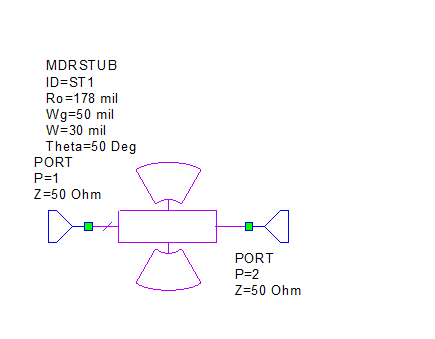
\includegraphics[scale=0.7]{radial_stub.png}
    \caption{The circuit schematic for the broadband radial stub filter at the mixer output.}
    \label{fig:radialstub}
\end{figure}

\begin{figure}[!htbp]
    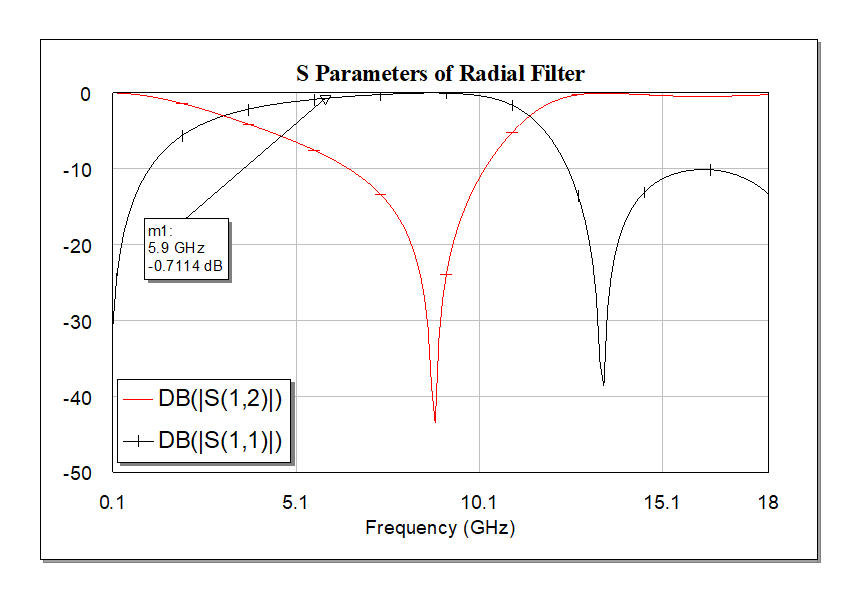
\includegraphics[scale=0.4]{filter_Sparams.png}
    \caption{The S parameters of the radial filter stub}
    \label{fig:radialparams}
\end{figure}

With the output filter network designed and optimized, we then designed the artwork for the diode package. The datasheet for the HSMS-8202 Avago anti-parallel diodes strongly guided the design considerations. The diode package in this case has three output pins for which we designed three pads. The pads were 35 mils wide and 80 mils long for ease of connection of the diode circuit to the mixer network. The three pads wer made from short sections of transmission line on Rodgers 3210. The diode model in MWO was constructed from the equivalent linear model given in the data sheet. The self-bias resistance $R_j$ was set to 146 $\Omega$. The schematic is shown in figure \ref{fig:diodemodel} with the simulated S parameters given in figure \ref{fig:diodeparams}. The diode package combining the two diode circuits into an equivalent matched diode pair is shown in figure \ref{fig:diodepackage}. 

\begin{figure}[!htbp]
    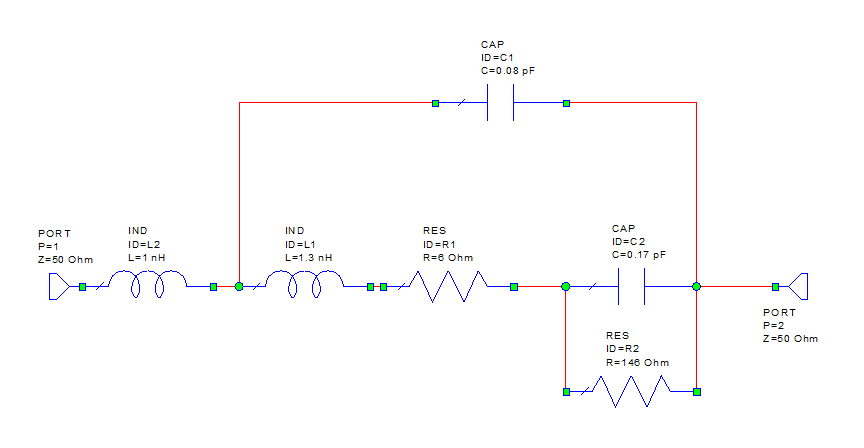
\includegraphics[scale=0.4]{diode_circuit.png}
    \caption{The equivalent linear diode circuit used to model the response of the diode in the mixer.}
    \label{fig:diodemodel}
\end{figure}

\begin{figure}[!htbp]
    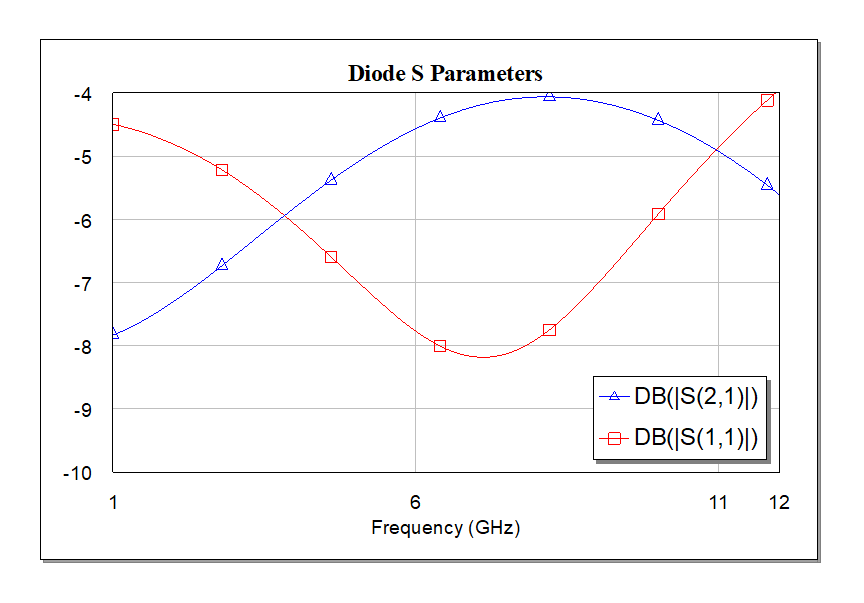
\includegraphics[scale=0.4]{diode_Sparams.png}
    \caption{The S parameters of the linear equivalent diode circuit model.}
    \label{fig:diodeparams}
\end{figure}

\begin{figure}[!htbp]
    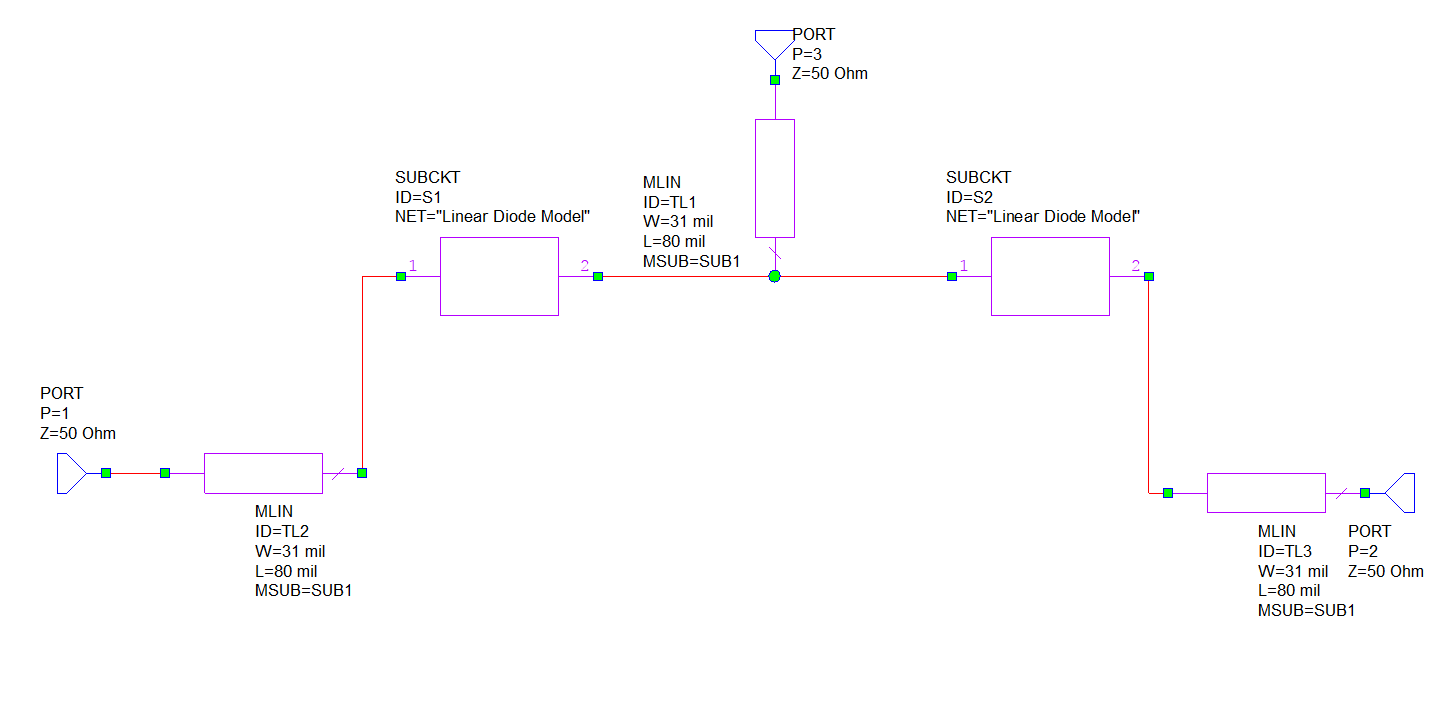
\includegraphics[scale=0.25]{diode_package_circuit.png}
    \caption{The package model for the diode showing the two diode circuits connected with short transmission line sections.}
    \label{fig:diodepackage}
\end{figure}


The diode model and the output filter network were then combined and simulated to obtain the reflection coefficient looking into the input of the network. We then designed input matching networks to bring the diode circuits to the 50 $\Omega$ impedance of the branch line coupler lines. The diode networks were well matched even with no additional matching circuits at their input. We decided to simply use 0 $\Omega$ resistors in place of any matching inductors.

There was no additional design work for the Branch Line Coupler above the designs from Lab 2. In lab 2, we achieved coupling to port 3 of -3.32 dB, insertion loss at port 2 of -3.04 dB, and an isolation at port 4 of -24.55 dB at 5.9 GHz. The response of the branch line circuit is shown in figure \ref{fig:branchparams}. With the branch line circuit completed, diode network and output and input matching subcircuits optimized, we combined all these parts into the full mixer network shown in figure \ref{fig:fullcircuit}.


\begin{figure}[!htbp]
    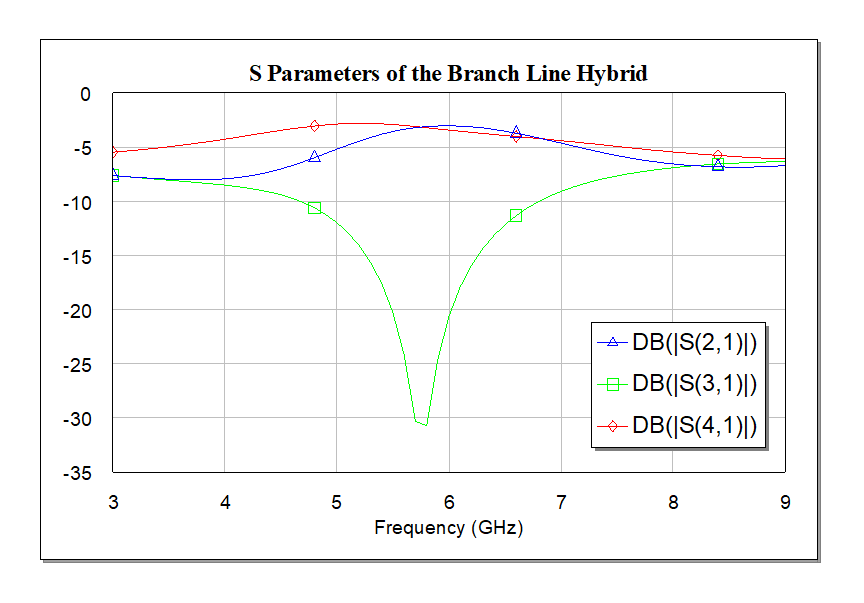
\includegraphics[scale=0.4]{BranchLine_Sparams.png}
    \caption{The S parameters of the Branch Line Coupler Hybrid for the mixer.}
    \label{fig:branchparams}
\end{figure}

\begin{figure*}[!htbp]
    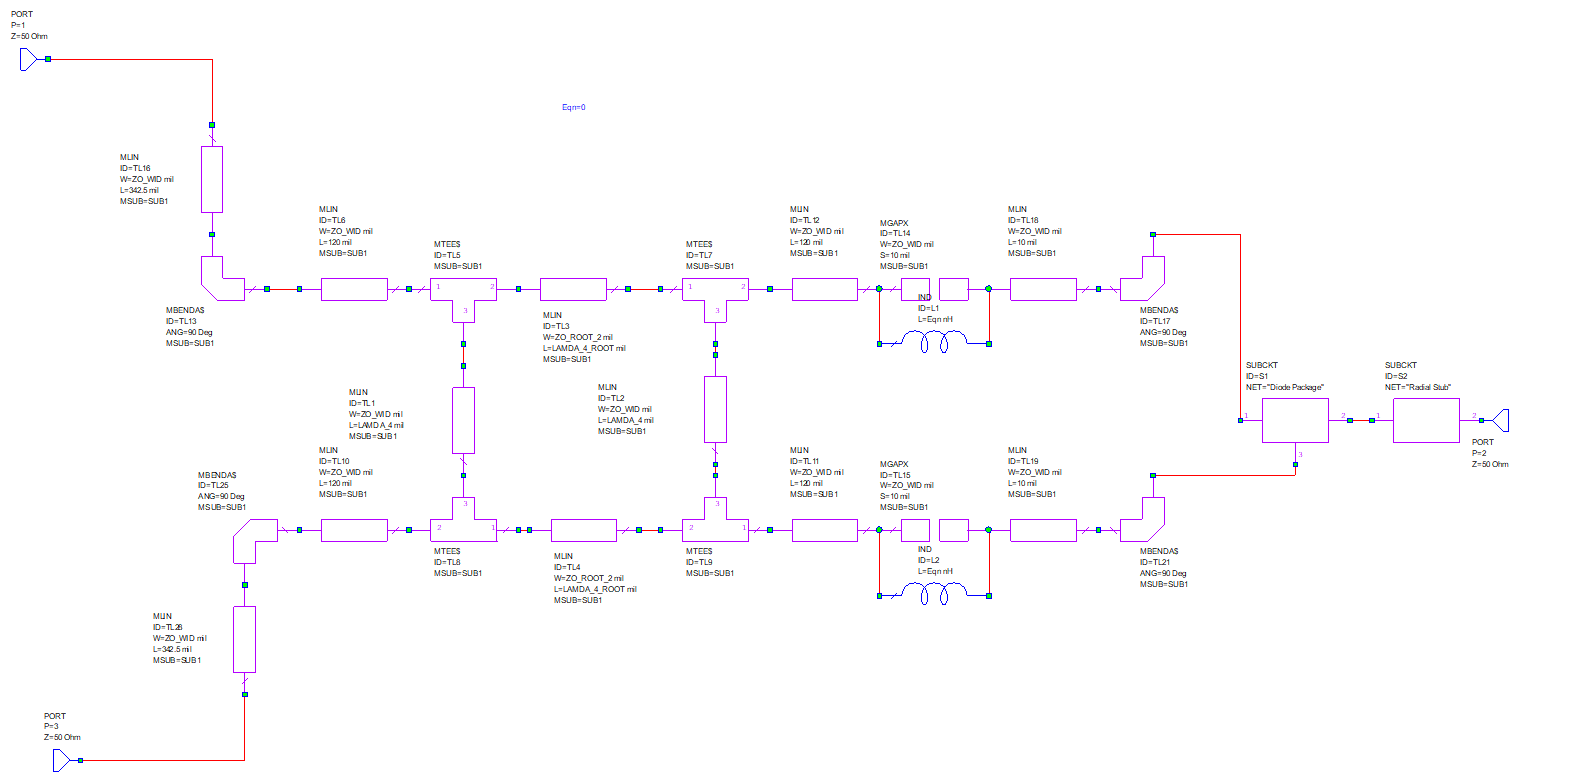
\includegraphics[scale=0.46]{full_circuit.png}
    \caption{The completed circuit schematic for the mixer network.}
    \label{fig:fullcircuit}
\end{figure*}


% \FloatBarrier

\section*{Lab Testing}

The first step of the in lab measurements was to calibrate the two signal generators. We used the Hittite HMC-T2220 signal generator to source the RF signal. A National Instruments Synthesizer was also provided as the LO source. Since the sources also generate power at additional frequencies due to their imperfections, we added bandpass VBFZ-55990S+ filters to the outputs of the RF and LO generators and calibrated the sources with the filters in place. The calibration of the Hittite signal generator was done to translate from the power at the source to the actual measured signal at the FFox. This accounts for losses in the cable and filters. Since we expect the losses to be constant with frequency (as long as the source frequency is within the bandpass), we only calibrated the RF generator at 5.89 GHz - a single frequency. We found that there was a 3.9 dB loss in signal from the source as measured on the FFox. The power output of the NI synthesizer used as the LO source was controlled by adjusting a digital step attenuation which can be controlled through a computer interface. Calibration thus allowed us to translate from attenuation of the source to the actual power measured at the FFox. We found an attenuation of 10 dB translated to 1.7 dBm power at the FFox.

With the sources properly calibrated, the RF and LO inputs were hooked to the inputs of the  mixer hybrid. The IF output of the mixer was then fed into the FFox Spectrum Analyzer (SA). The setup is shown in figure \ref{fig:setup}.We set the RF power to -20 dBm while the LO power was set to 3dBm. The LO frequency was initially set to 5.89 GHz while the RF output was at 5.9GHz. The IF signal as measured on an oscilloscope is shown in figure \ref{fig:oscilloscope}
\begin{figure}[!htbp]
    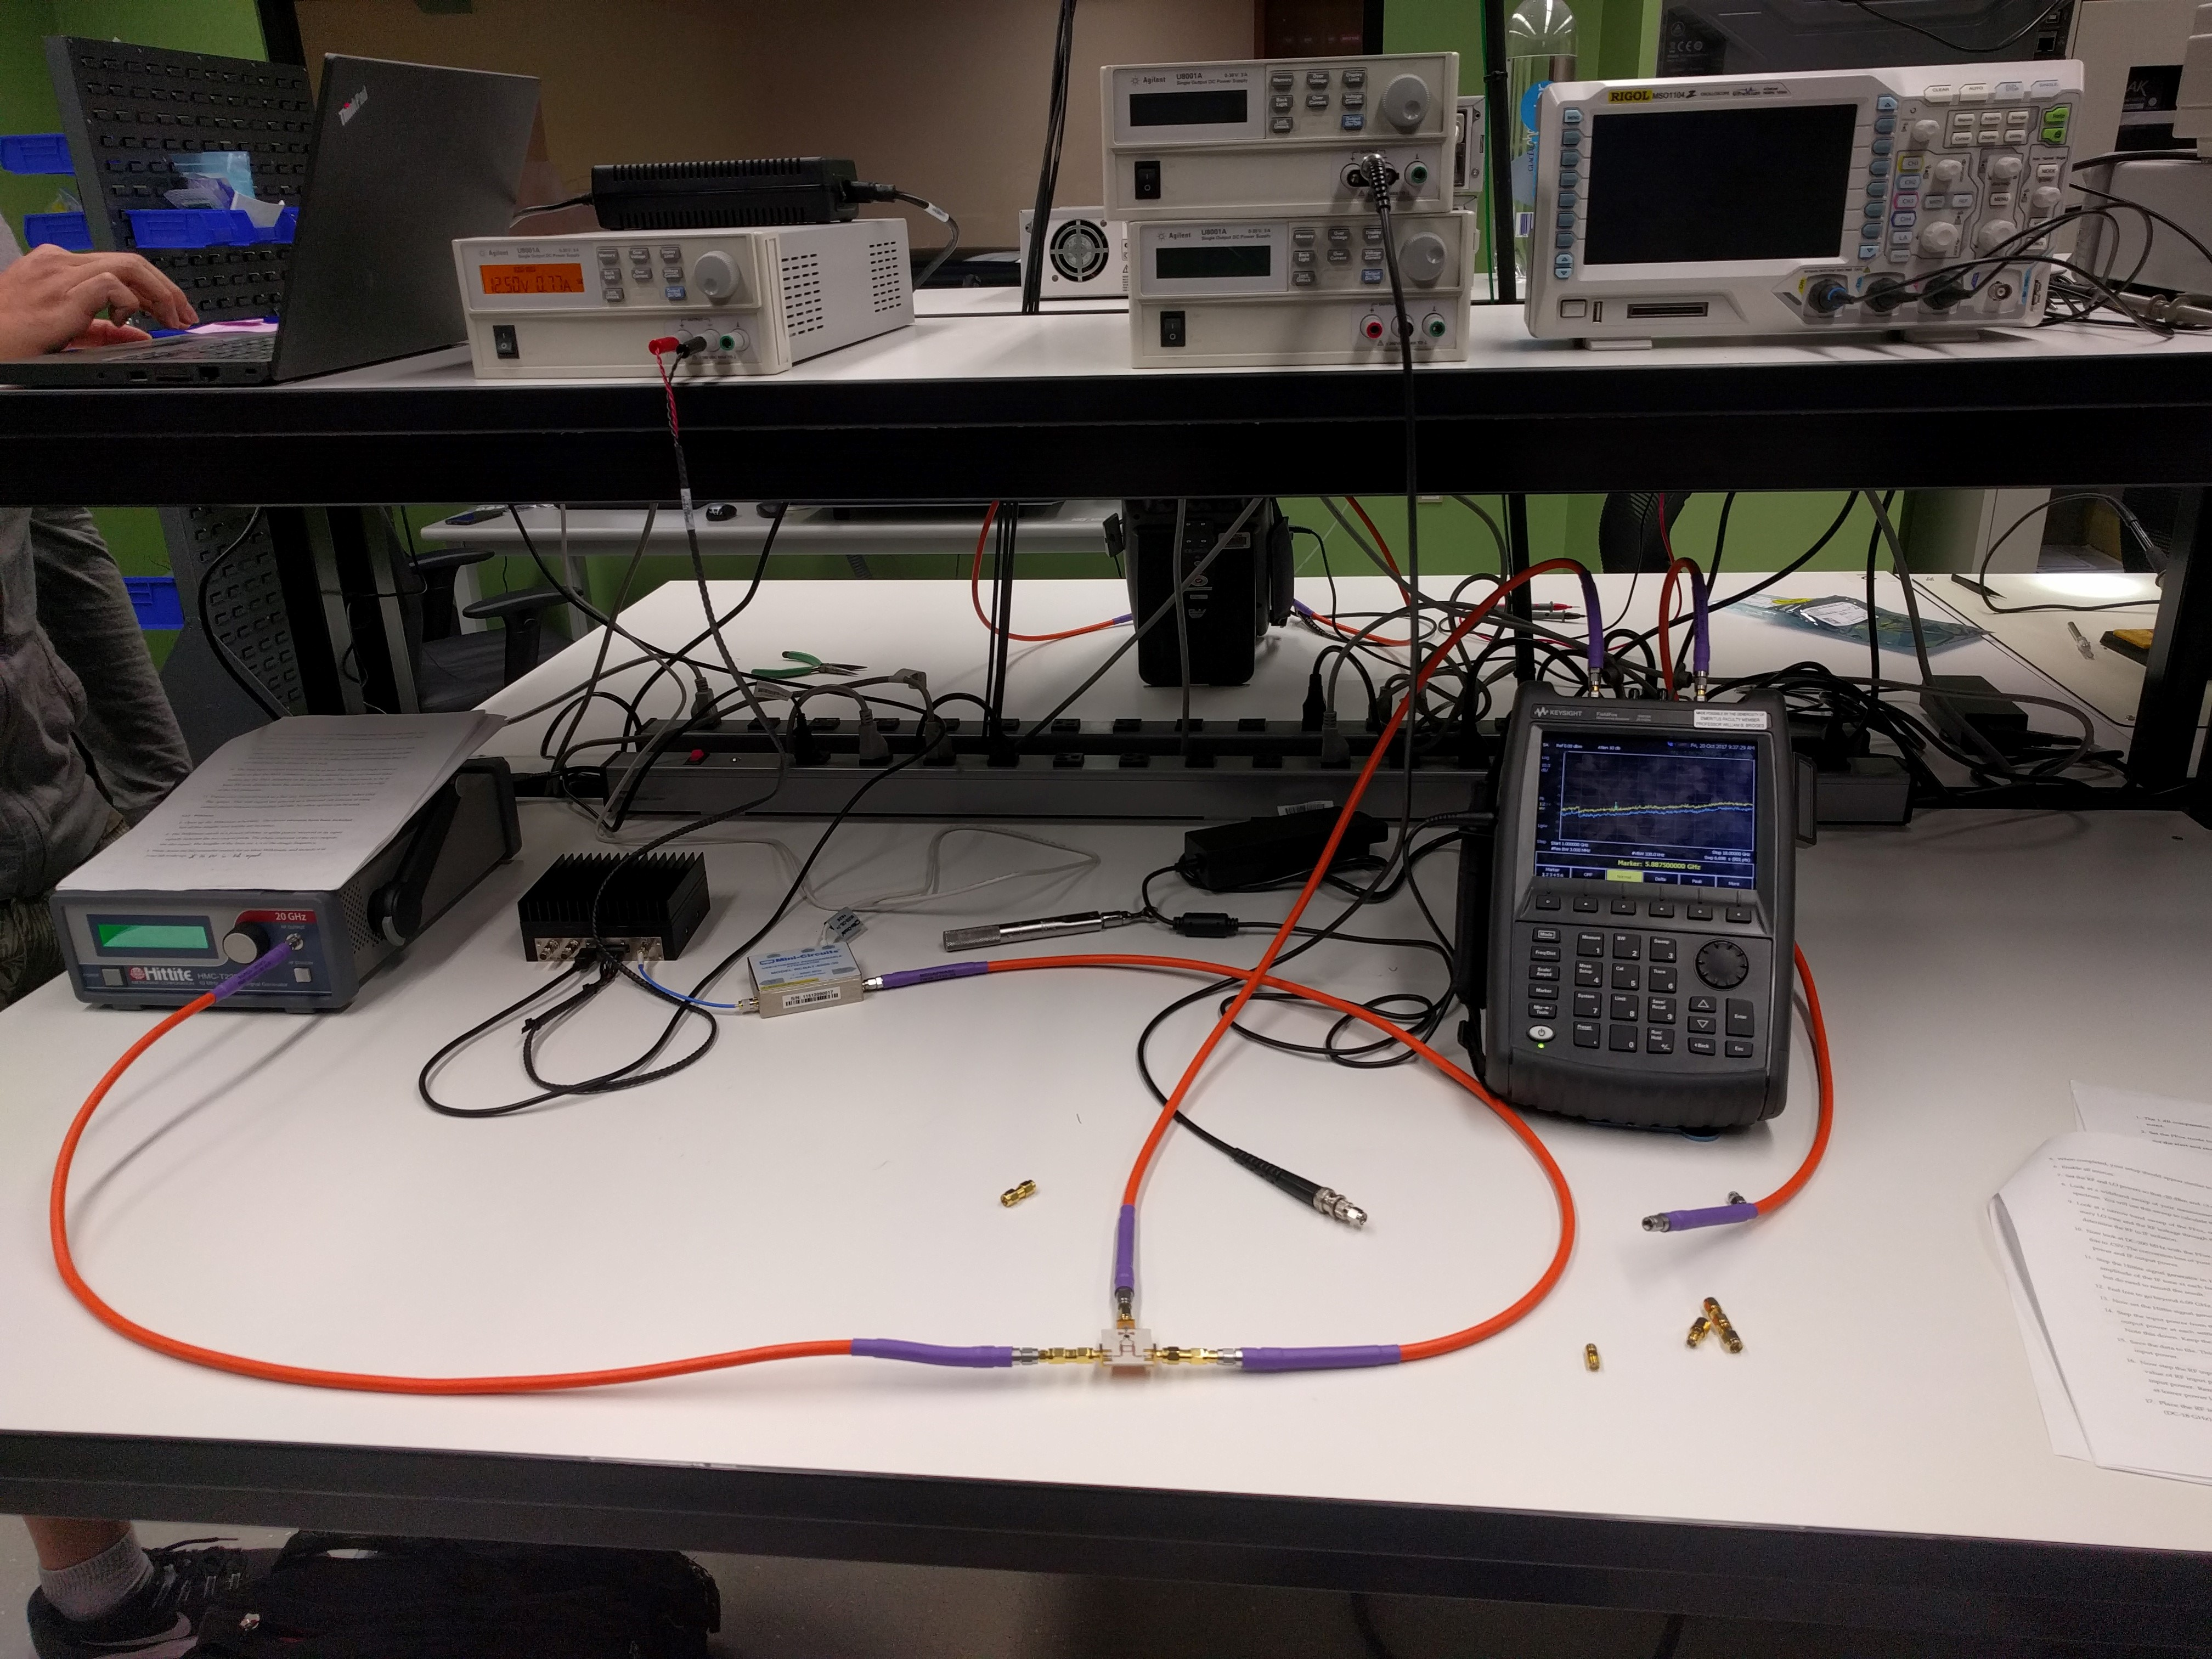
\includegraphics[scale=0.05]{setup.jpg}
    \caption{The mixer circuit interfaced with the FFox and the RF and LO signal sources.}
    \label{fig:setup}
\end{figure}


\begin{figure}[!htbp]
    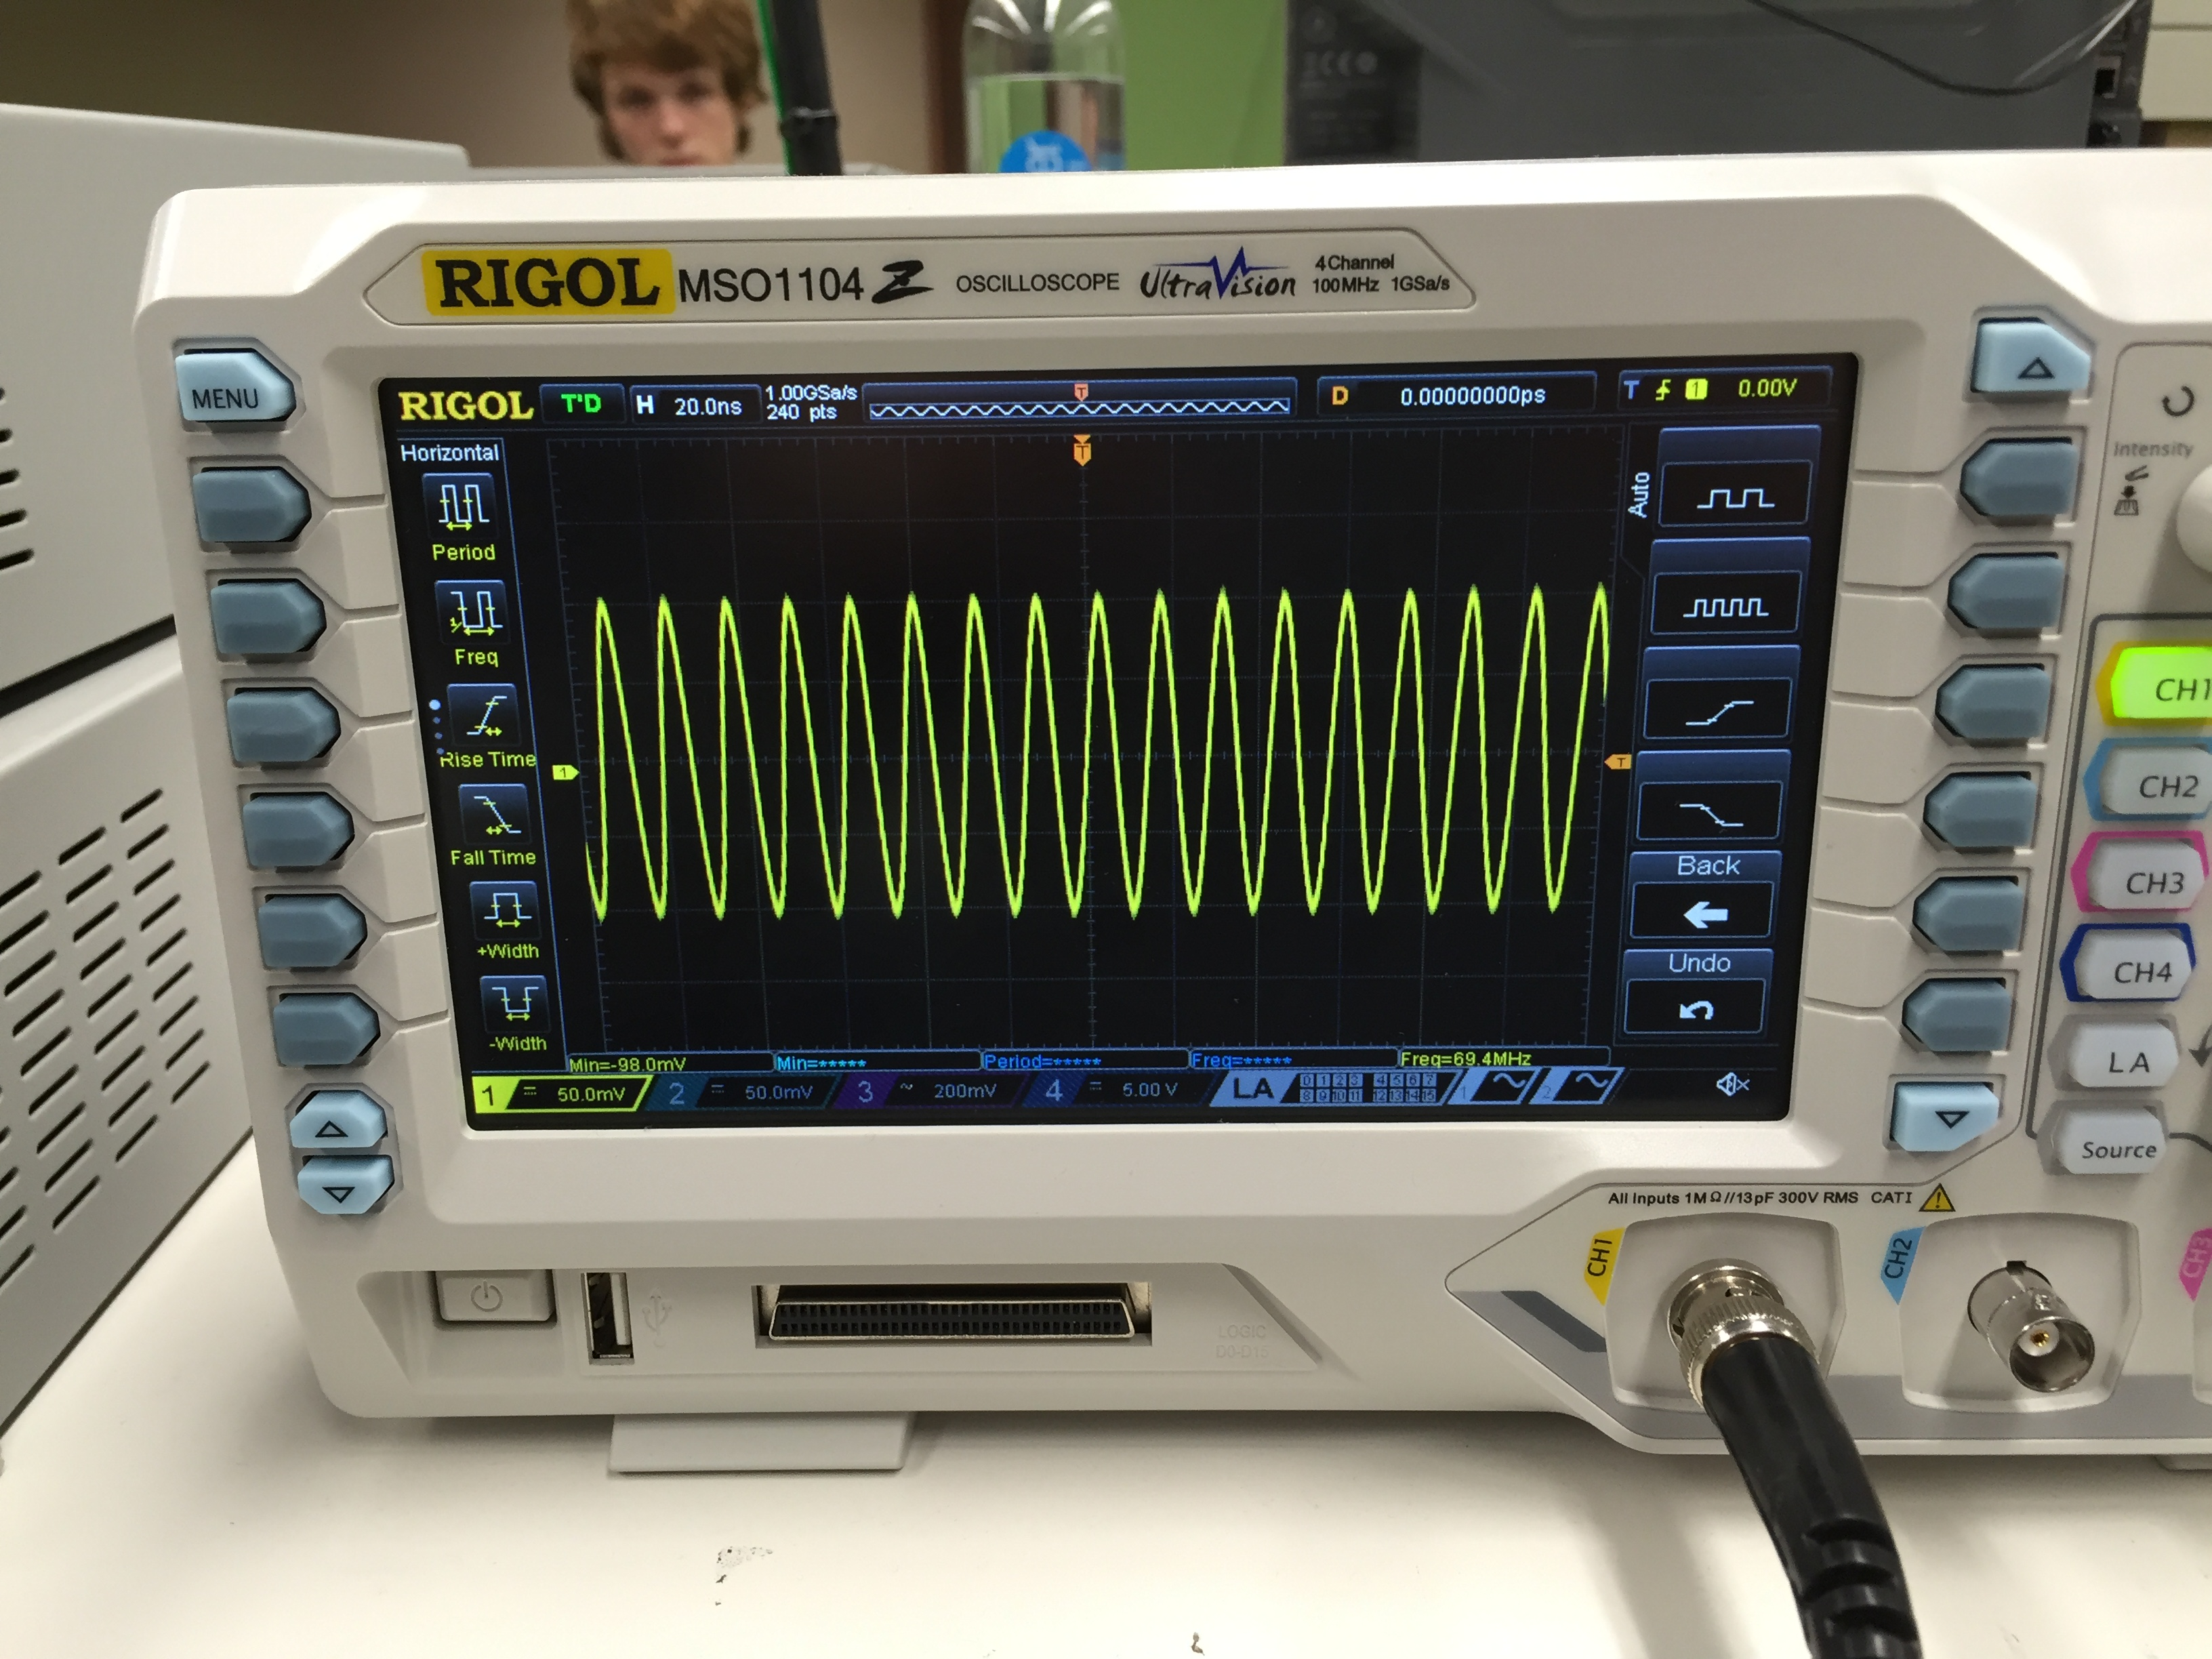
\includegraphics[scale=0.06]{oscilloscope.jpeg}
    \caption{IF power measured on the oscilloscope.}
    \label{fig:oscilloscope}
\end{figure}

A number of different measurements were performed to obtain the Conversion Loss, LO to IF isolation , RF to IF isolation as well as the impact of LO and RF power on the IF signal strength. We first performed a wideband sweep of the SA. This revealed several products at not only the IF frequency, but also at the LO and RF frequencies as well as at high harmonics. We also made narrower band measurements centered about the RF frequency to measure the RF leakage at the IF port. In the circuit design, the radial stub filter at the output was designed to suppress this leakage. A narrow band measurement at the IF frequency was made to determine the conversion loss of the filter. With the initial choices of LO and RF frequencies, the IF signal was at 10 MHz. However, we noted that there was much high conversion efficiency at very low frequencies. Other groups also reported the same behavior of the mixer circuit. As a result, we adjusted the LO to a 5.8 GHz output to give a 100 MHz IF frequency. 

We also measured the response of the mixer to stepping the LO input power. To do so, we adjusted the LO power in 1 dB steps from -5 dBm to +7 dBm  and found that the IF power was highest at LO power of 3 dBm. This gave the optimal conversion loss for our mixer network. We set this as the LO power level for the rest of the measurements.

The RF power was also stepped from -30 dBm to 0 dBm and the IF power output recorded. From the measurements, it was clear that the conversion loss was constant at lower RF input power and increased at higher RF power levels. This gave us a measure of the linearity of the mixer response. This is further discussed in section \ref{sec:analysis}.

We reset the RF power to -20 dBm and the RF frequency to 5.85 GHz. We made a wide band measurement of the mixer from DC-18GHz. This measurement was used to characterize the level of the 1st harmonic of the RF and LO signals. Lastly, we made a narrow band measurement from 5.7 - 6.1 GHz to better measure the RF leakage at the IF output.

\FloatBarrier
\section*{Analysis}\label{sec:analysis}

The figure \ref{fig:IFoutput} shows the IF signal measured at the output of the mixer with the RF at 5.9 GHz. The IF peak is at 100 MHz while a smaller peak at 180 MHz is also visible. The source of this peak is unknown as it was not present in all the measurements made at the lower frequencies. To obtain the peak IF power, we fitted the peak to a quadratic as shown in figure \ref{fig:IFoutputfitted}. The peak IF power was found to be -31.26 dBm. With the -20 dBm RF input this gives a -11.26 dBm conversion loss of the mixer.

\begin{figure}[!htbp]
    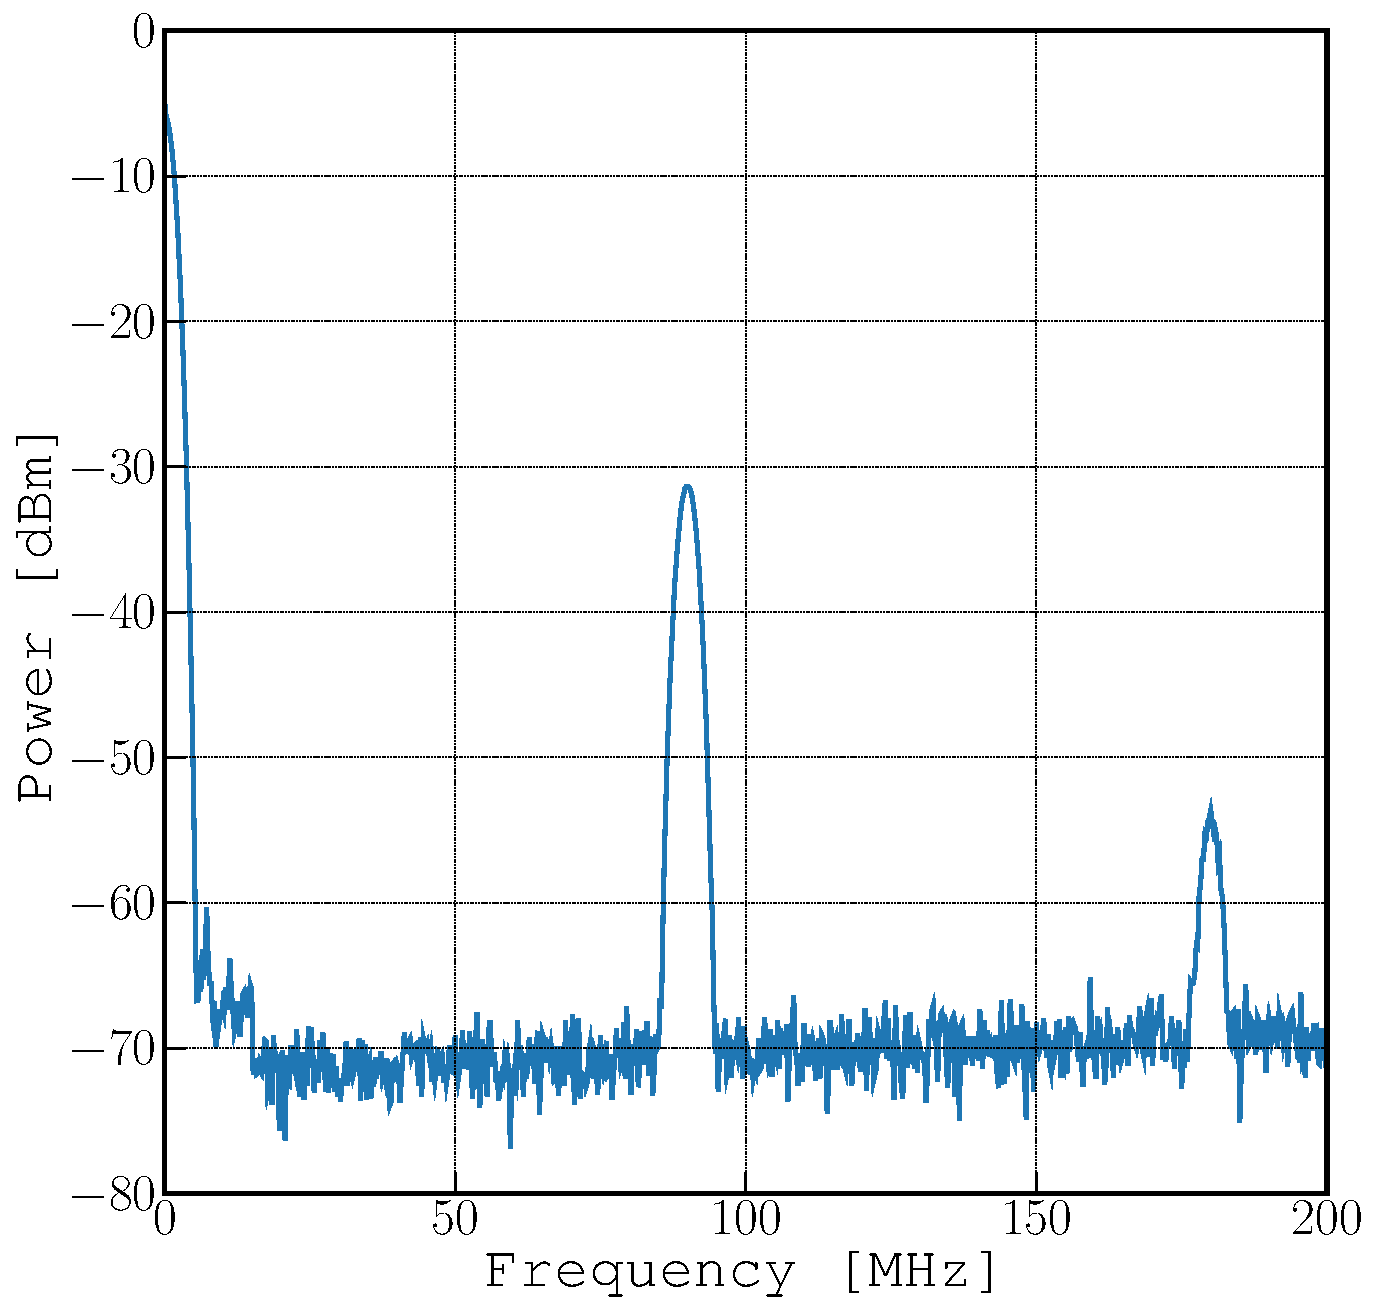
\includegraphics[scale=0.35]{DC_to_200MHz.pdf}
    \caption{Low Frequency Spectral response of the mixer showing the mixer output at 100 MHz.}
    \label{fig:IFoutput}
\end{figure}

\begin{figure}[!htbp]
    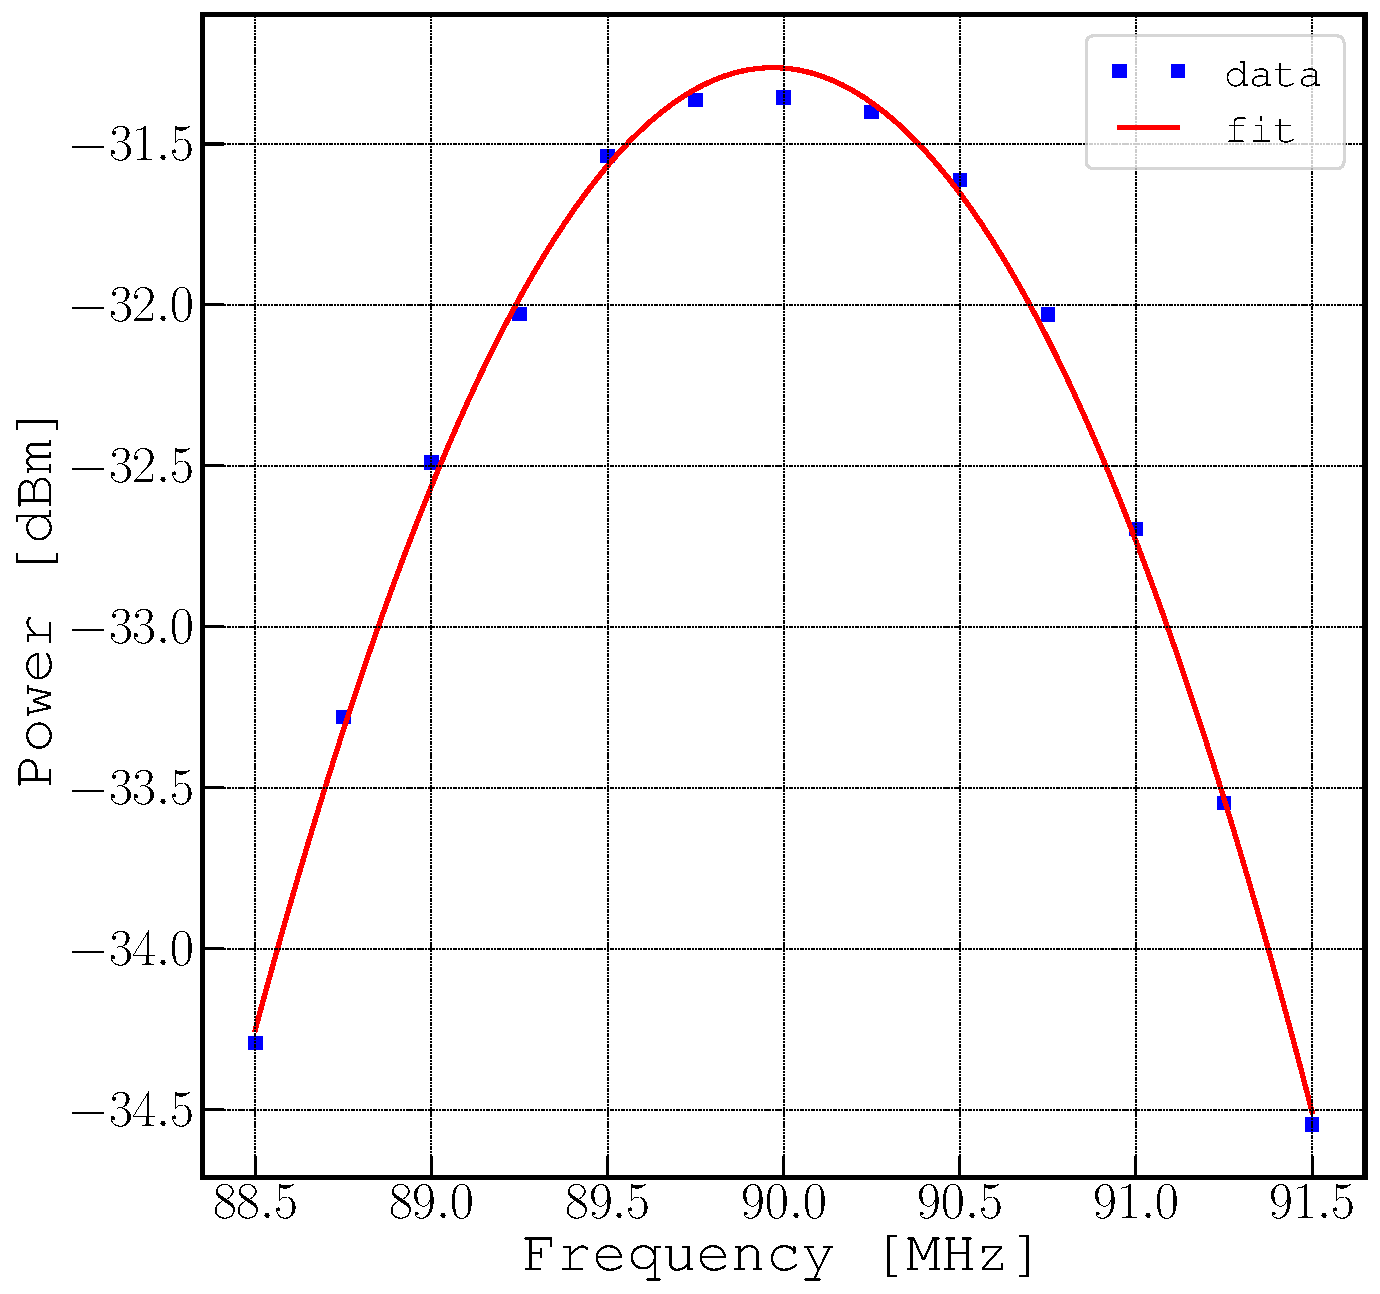
\includegraphics[scale=0.35]{DC_to_200MHz_zoomed.pdf}
    \caption{A fit to the IF peak to more accurately determine the conversion loss of the mixer.}
    \label{fig:IFoutputfitted}
\end{figure}

We determined the conversion loss as a function of the RF frequency from the RF frequency sweep. The results are plotted in figure \ref{fig:CLvsRFfrequency}. From the figure, we see that the response of the mixer is broadband over a wide frequency range from 5.7 - 6.1 GHz. However, there is a rippling effect in the passband of the mixer. The ripple amplitude is about 2 dB. The lowest conversion loss measured for this mixer was 8.72 dB at 5.97 GHz. Below about 5.85 GHz, the conversion loss rapidly increases. Thus the lower end of the mixer bandpass is at about 5.85 GHz. We did not further explore the upper limits of the mixer passband since it was beyond our measurement range of interest.

\begin{figure}[!htbp]
    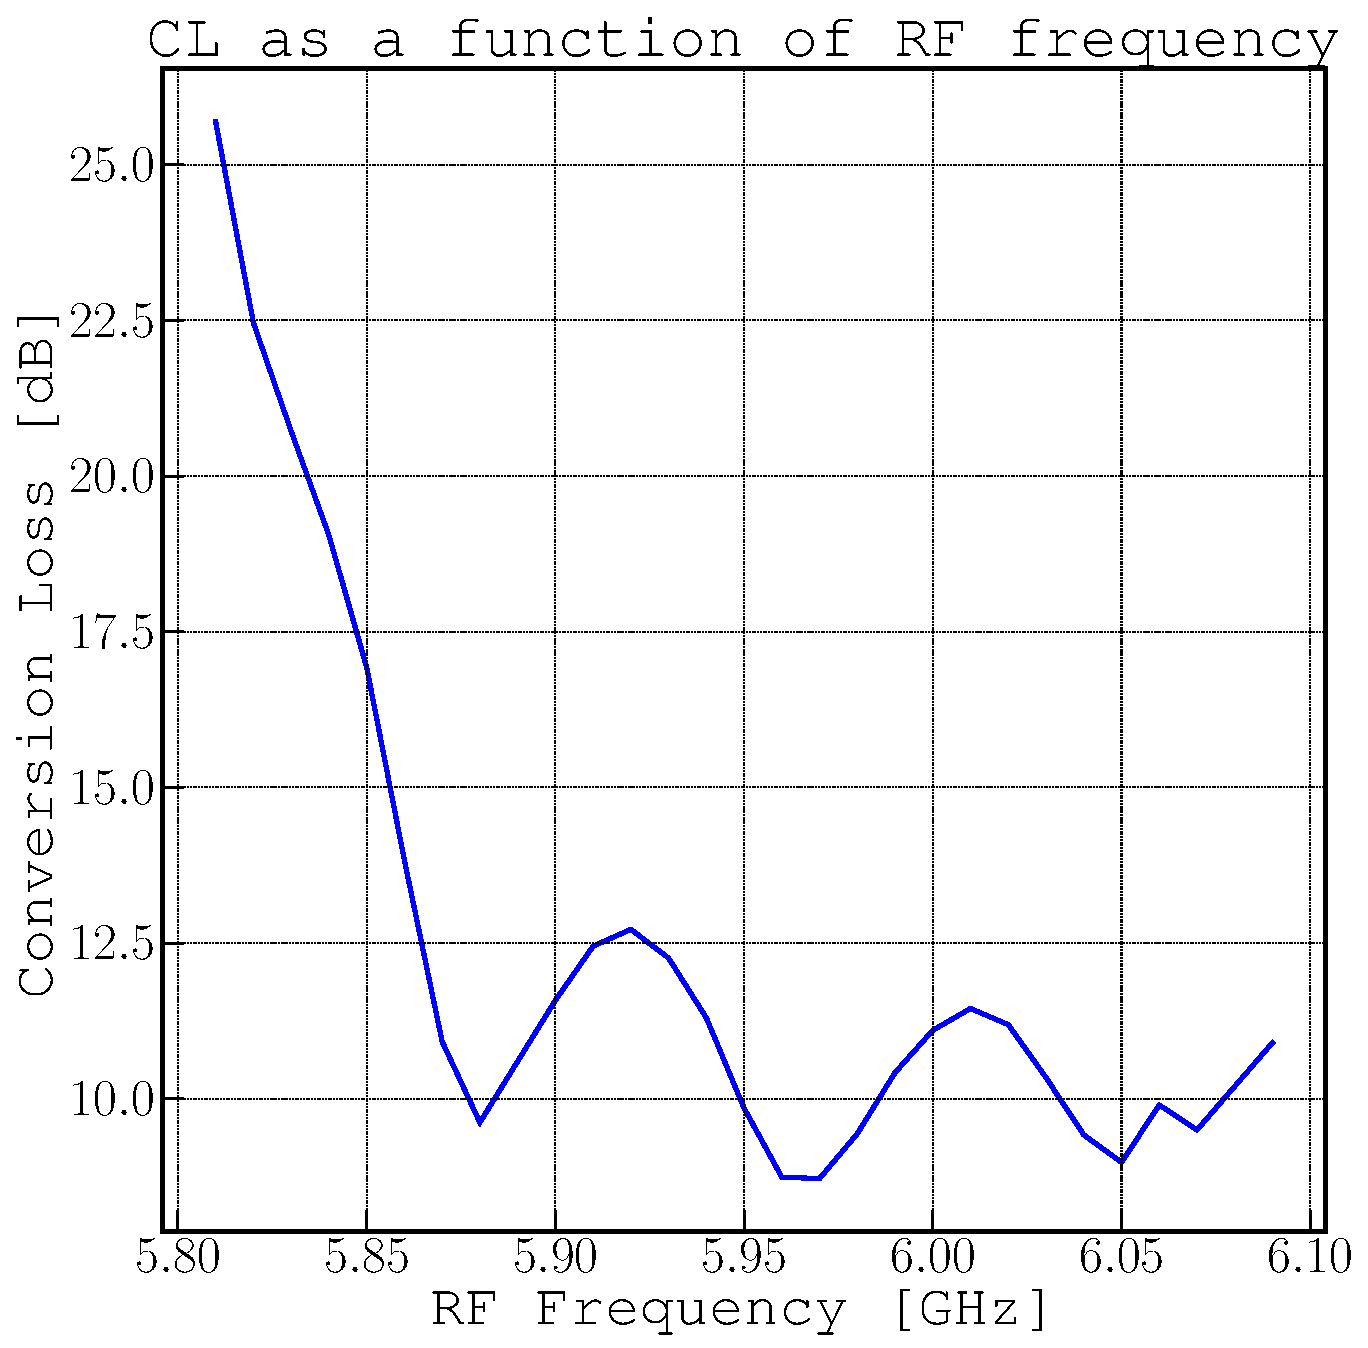
\includegraphics[scale=0.35]{CL_vs_RF_frequency.pdf}
    \caption{The CL as a function of the RF frequency. The mixer response is high above 5.7 GHz.}
    \label{fig:CLvsRFfrequency}
\end{figure}

When the conversion loss is plotted as a function of the LO power as shown in figure \ref{fig:CLvsLOpower}, we found that the CL is minimized at an LO power of 3 dBm. For the RF power equal to -20 dBm, this gives the optimal CL of 11.52 dB at 5.9 GHz. The manufacturer's specification given in the datasheet which shows the diode have a minimized CL at 2 dBm LO power. However taking into account that the branch line couple splits the input power providing three 3dB power to each of the diodes, this corresponds to a 5 dBm LO input power. Our optimal LO power is therefore lower than the specified level from the manufacturer. This deviation is likely a result of the limitations of the branch line circuit. If the branch line coupler delivers slightly different power levels to its two outputs then the net effect would be that the optimal CL will be achieved at lower LO power levels at the input. 

\begin{figure}[!htbp]
    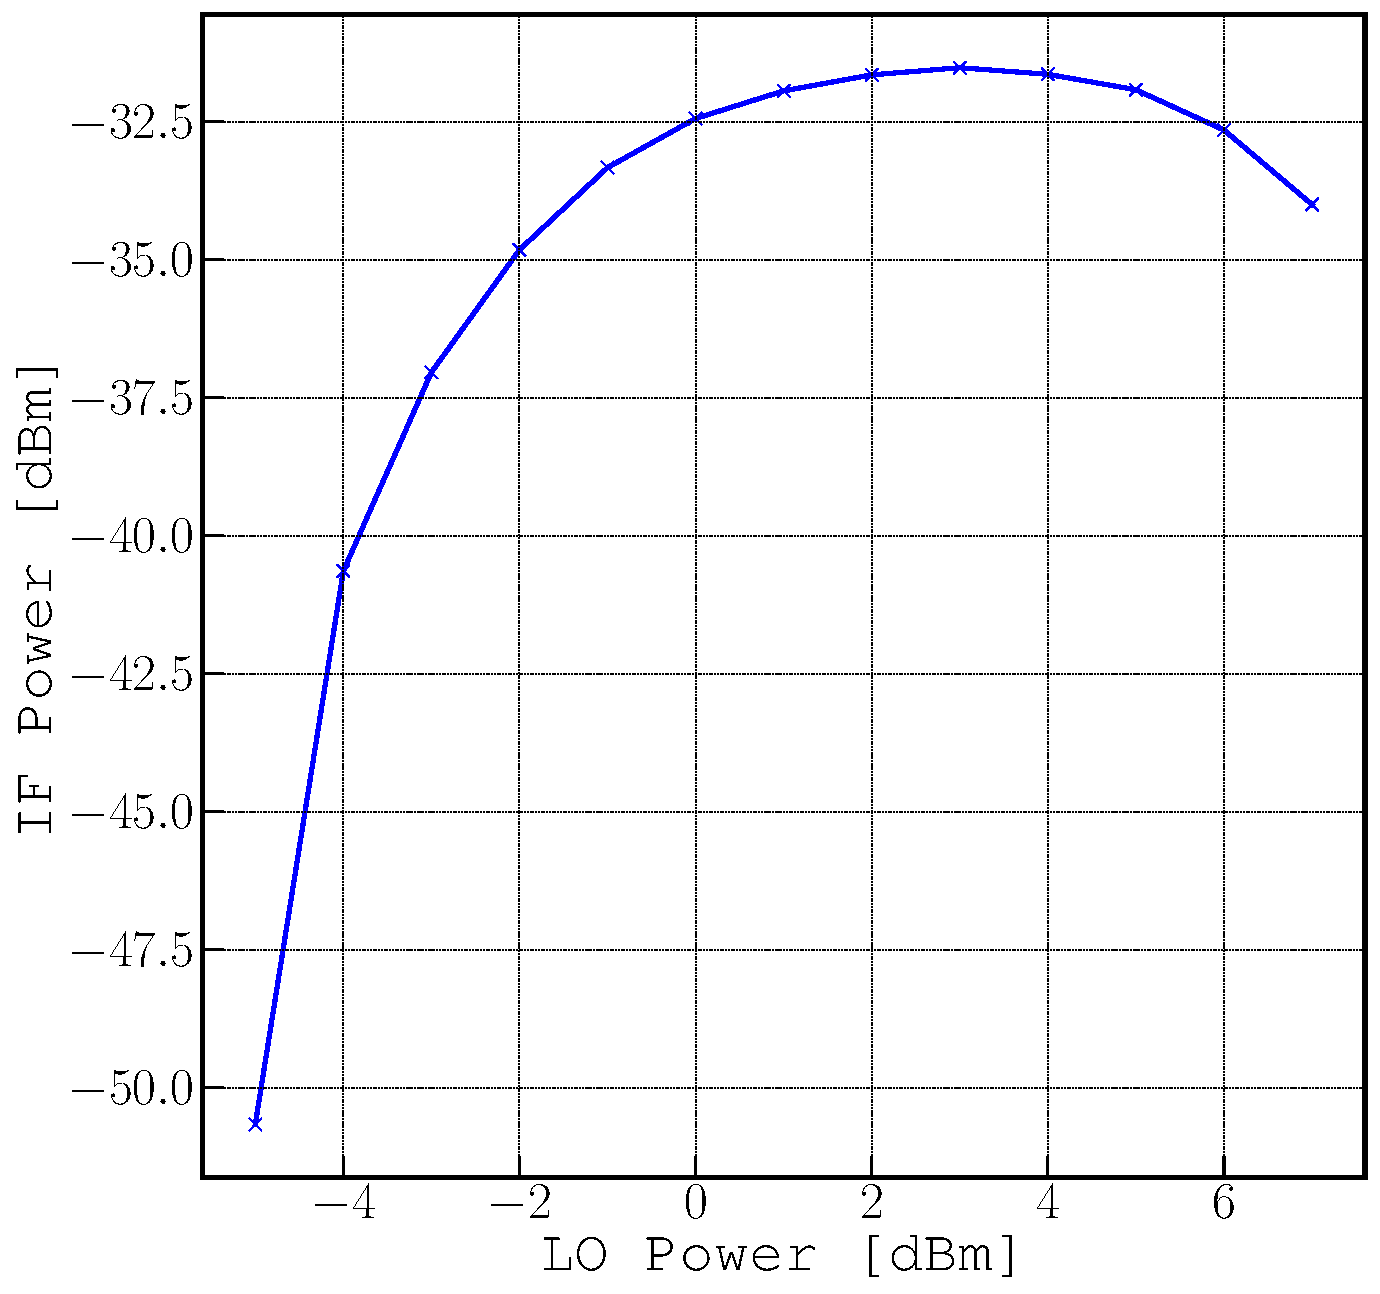
\includegraphics[scale=0.35]{IF_Power_vs_LO_power.pdf}
    \caption{The Conversion Loss as a function of the LO power.}
    \label{fig:CLvsLOpower}
\end{figure}

We also explored the conversion loss as a function of the RF power as shown in figure \ref{fig:compressionpoint}. From the figure, it is clear that at low RF power levels, the conversion loss is constant but sharply increases at higher frequencies. We fitted the data for RF powers less than -20 dBm to a linear fit and found that CL = 11.68 dB well described the data as shown in the figure. The slope of the line was found to be 0.01 consistent with having a constant CL over the entire linear regime. The 1 dB compression point of the mixer was found to be at RF powers between -10 and -11 dBm. 


\begin{figure}[!htbp]
    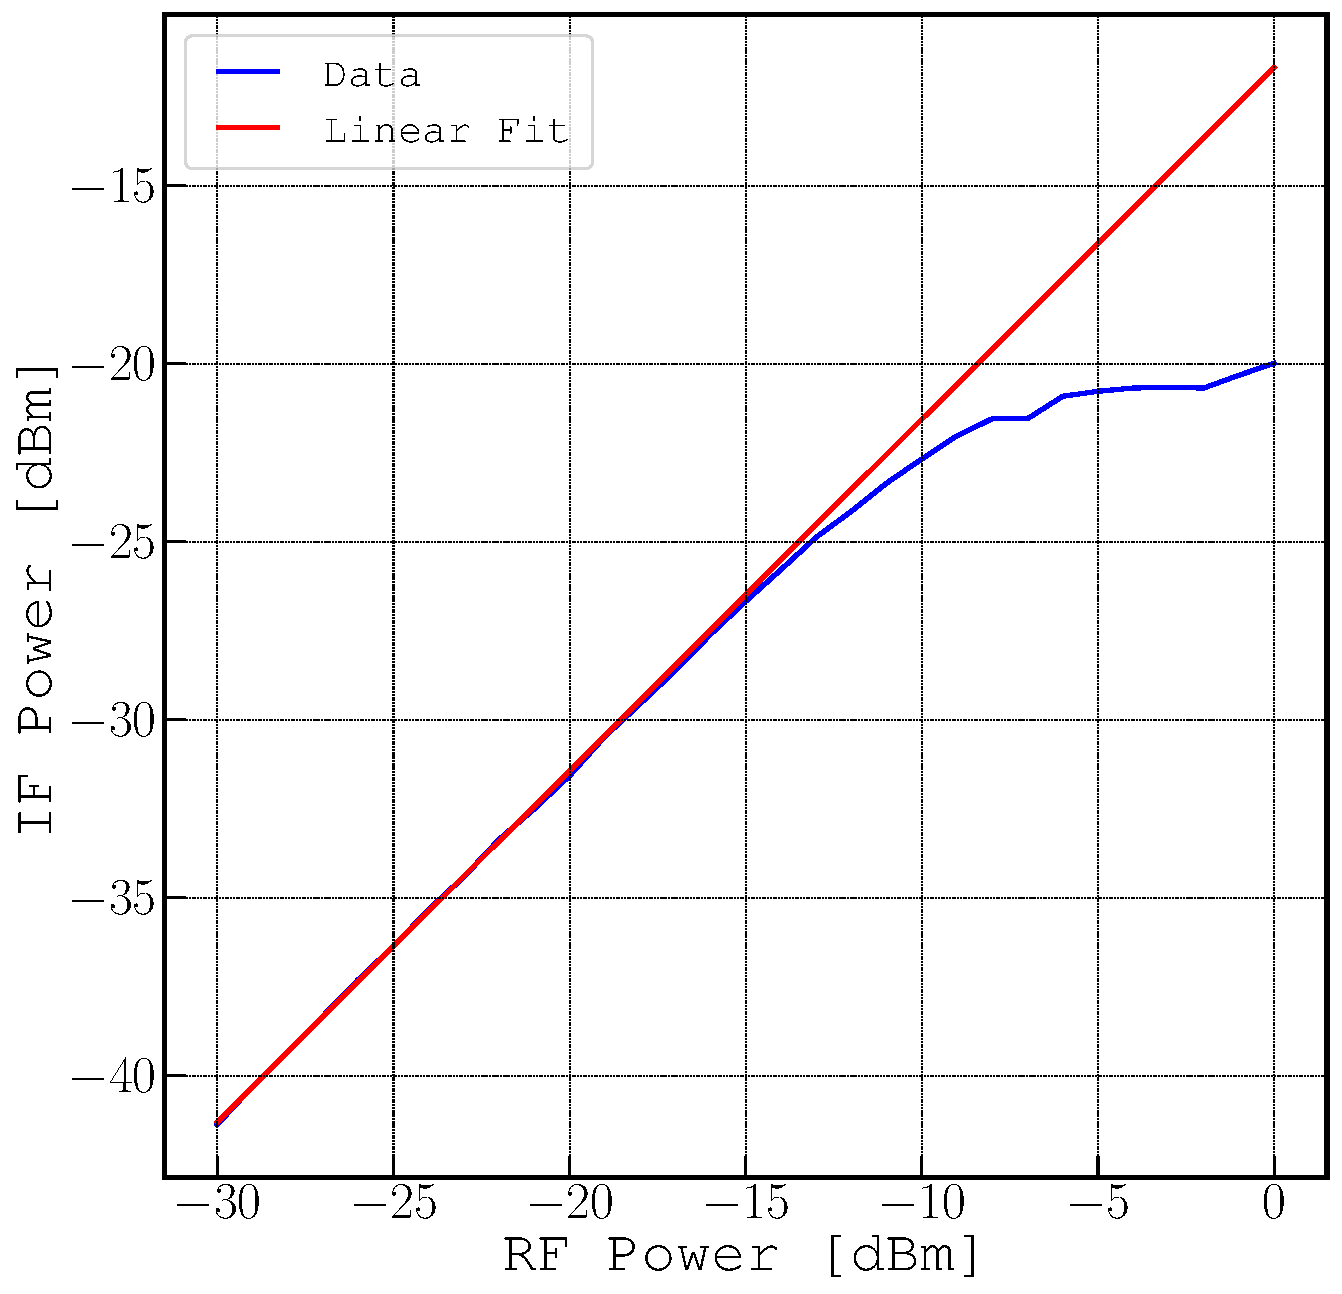
\includegraphics[scale=0.35]{compression_point_fitted.pdf}
    \caption{The conversion loss as a function of the RF power. At low RF power, there is good agreement between the measured RF power and the linear fit to the conversion loss.}
    \label{fig:compressionpoint}
\end{figure}


We were also interested in characterizing the spectral leakage of the mixer. The figure \ref{fig:wideband} shows a DC to 18 GHz sweep of the mixer. At the lower frequencies, there is a strong signal at DC and at 200 MHz. There is a strong peak at 5.8 GHz due to the LO power leakage at the mixer output as well as a RF peak at 5.85 GHz. Additionally, we have strong first harmonics of the LO and RF at 11.8 and 11.7 GHz respectively. The LO even shows a second harmonic at 17.6 GHz. With the LO power at 3 dBm, we measured the LO fundamental at the IF output as -5.99 dBm  while the first harmonic was at -19.36 dBm. The first harmonic was therefore at about 13.37 dBc. The LO isolation at the IF port was determined to be -8.99 dB.

\begin{figure}[!htbp]
    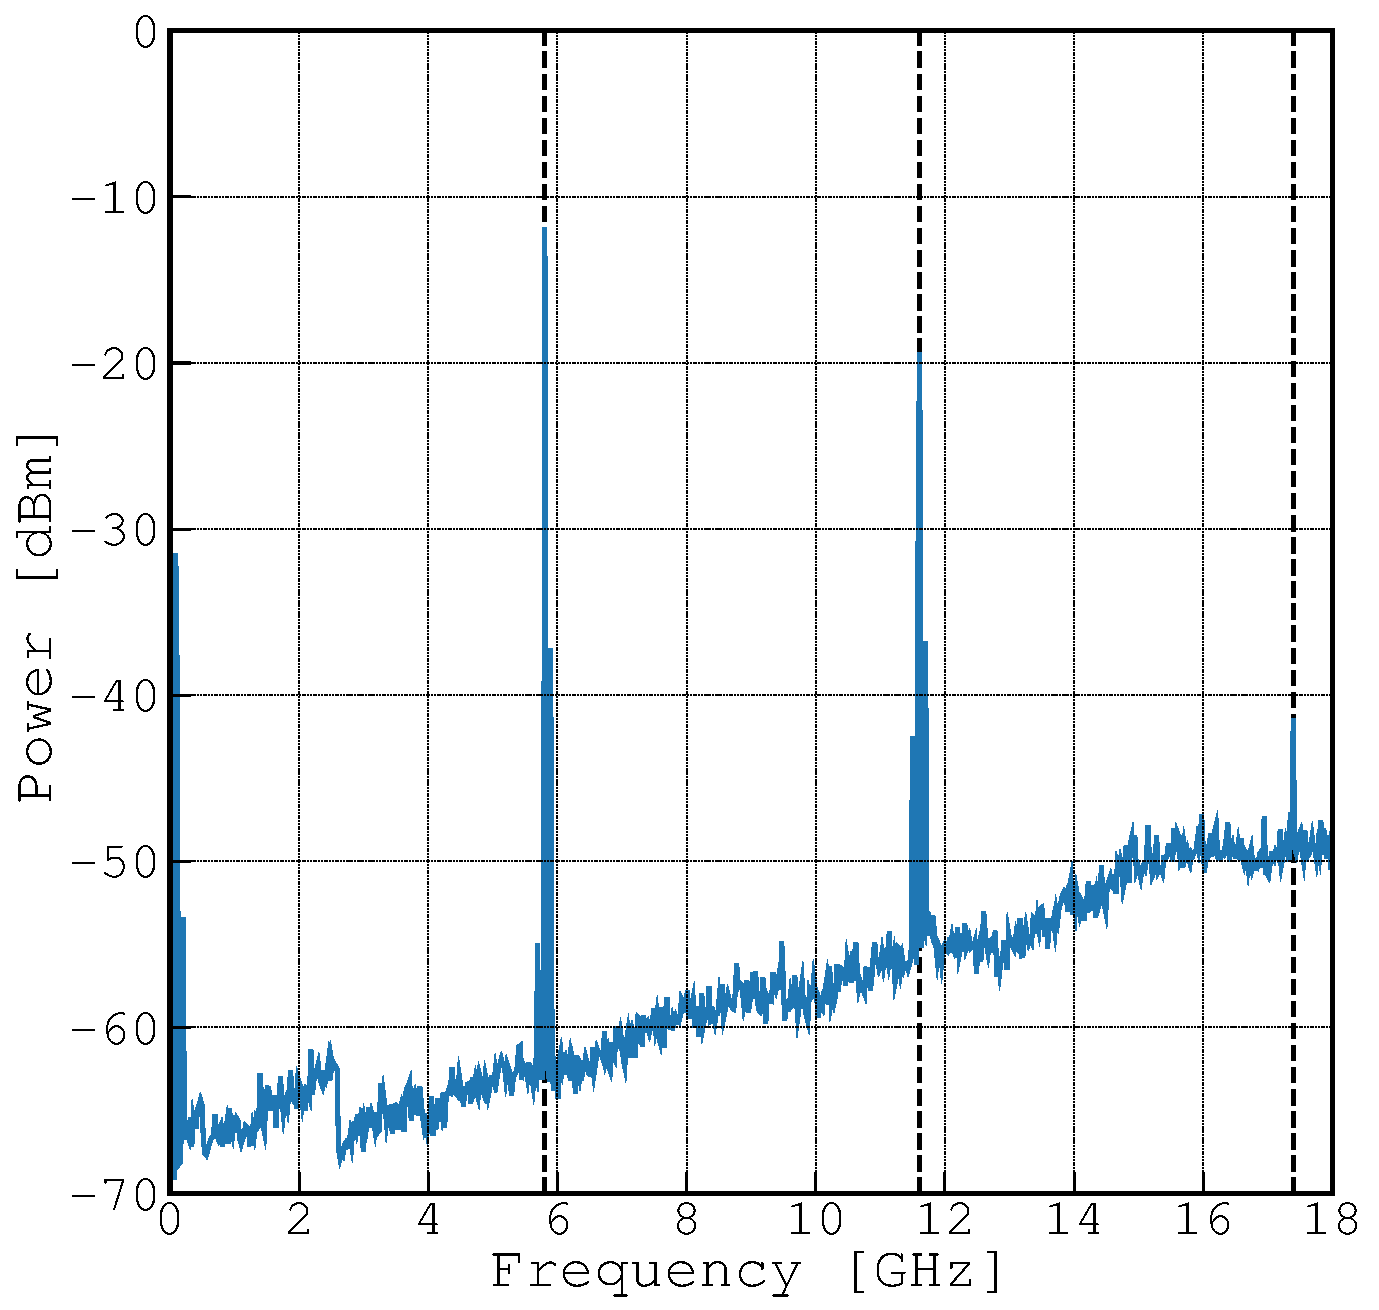
\includegraphics[scale=0.35]{DC_to_18GHz.pdf}
    \caption{Wide band response of the mixer. The black dotted lines show the LO fundamental and the first and second harmonics.}
    \label{fig:wideband}
\end{figure}

In addition, we measured the RF leakage power at the IF output. With the RF frequency at 5.9 GHz, we measured a peak RF power of -36.88 dBm as shown in figure \ref{fig:RFleakage}. Given the RF input signal power of -20 dBm, this corresponds to a -16.88 dB RF isolation at the IF port. 

\begin{figure}[!htbp]
    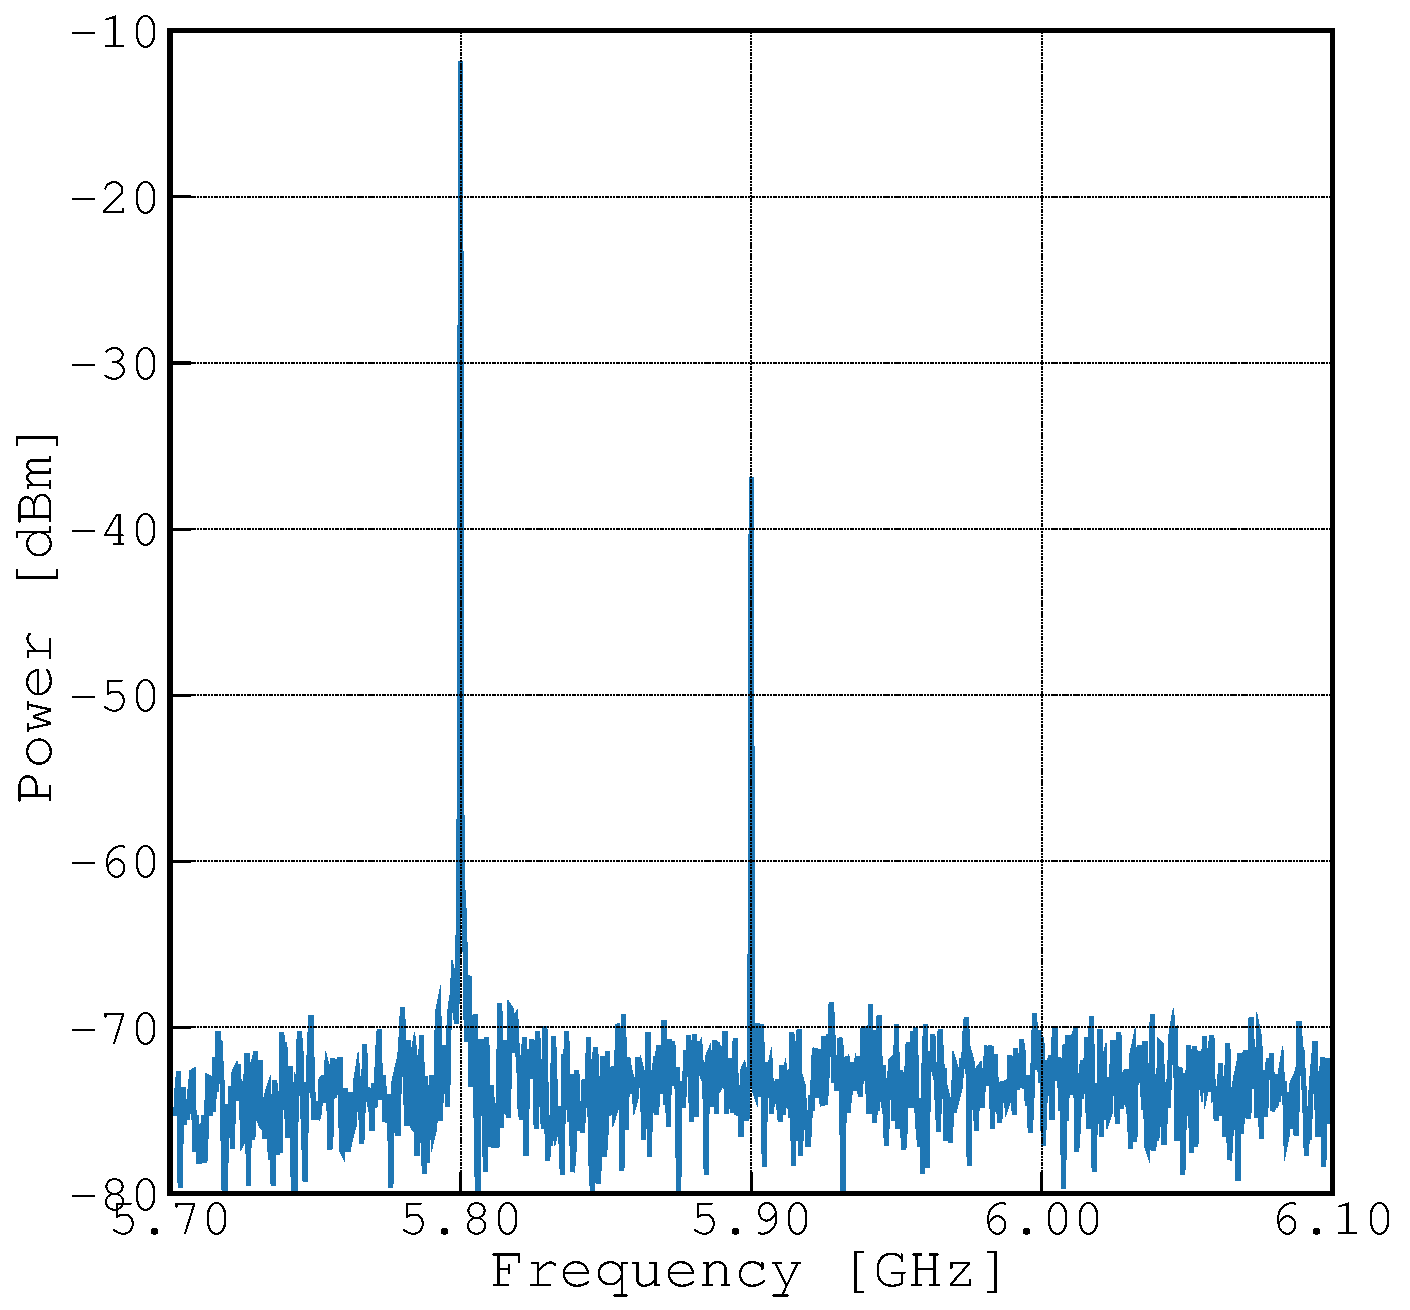
\includegraphics[scale=0.35]{RF_leakage.pdf}
    \caption{Narrow band measurement showing the LO peak at 5.8 GHz and the RF peak at 5.9 GHz.}
    \label{fig:RFleakage}
\end{figure}


\section*{Conclusions}
In this lab, we designed a mixer circuit that was able to achieve a conversion loss of 8.7 dB at RF frequencies of 5.95 GHz. We were also able to characterize the RF and LO isolation at the IF port as well as explore the effects of higher order harmonics in the mixer circuit. This lab well integrated the branch line concepts from lab 2.
\end{document}